\documentclass[
11pt, % The default document font size, options: 10pt, 11pt, 12pt
%oneside, % Two side (alternating margins) for binding by default, uncomment to switch to one side
english, % ngerman for German
singlespacing, % Single line spacing, alternatives: onehalfspacing or doublespacing
%draft, % Uncomment to enable draft mode (no pictures, no links, overfull hboxes indicated)
%nolistspacing, % If the document is onehalfspacing or doublespacing, uncomment this to set spacing in lists to single
%liststotoc, % Uncomment to add the list of figures/tables/etc to the table of contents
%toctotoc, % Uncomment to add the main table of contents to the table of contents
%parskip, % Uncomment to add space between paragraphs
%nohyperref, % Uncomment to not load the hyperref package
headsepline, % Uncomment to get a line under the header
%chapterinoneline, % Uncomment to place the chapter title next to the number on one line
%consistentlayout, % Uncomment to change the layout of the declaration, abstract and acknowledgements pages to match the default layout
]{MastersDoctoralThesis} % The class file specifying the document structure

\usepackage[utf8]{inputenc} % Required for inputting international characters
\usepackage[T1]{fontenc} % Output font encoding for international characters

\usepackage{mathpazo} % Use the Palatino font by default

\usepackage[backend=bibtex,style=authoryear,natbib=true]{biblatex} % Use the bibtex backend with the authoryear citation style (which resembles APA)

\addbibresource{example.bib} % The filename of the bibliography

\usepackage[autostyle=true]{csquotes} % Required to generate language-dependent quotes in the bibliography

%----------------------------------------------------------------------------------------
%	MARGIN SETTINGS
%----------------------------------------------------------------------------------------

\geometry{
	paper=a4paper, % Change to letterpaper for US letter
	inner=2.5cm, % Inner margin
	outer=3.8cm, % Outer margin
	bindingoffset=.5cm, % Binding offset
	top=1.5cm, % Top margin
	bottom=1.5cm, % Bottom margin
	%showframe, % Uncomment to show how the type block is set on the page
}

%----------------------------------------------------------------------------------------
%	THESIS INFORMATION
%----------------------------------------------------------------------------------------

\thesistitle{Thesis Title} % Your thesis title, this is used in the title and abstract, print it elsewhere with \ttitle
\supervisor{Dr. James \textsc{Smith}} % Your supervisor's name, this is used in the title page, print it elsewhere with \supname
\examiner{} % Your examiner's name, this is not currently used anywhere in the template, print it elsewhere with \examname
\degree{Doctor of Philosophy} % Your degree name, this is used in the title page and abstract, print it elsewhere with \degreename
\author{John \textsc{Smith}} % Your name, this is used in the title page and abstract, print it elsewhere with \authorname
\addresses{} % Your address, this is not currently used anywhere in the template, print it elsewhere with \addressname

\subject{Biological Sciences} % Your subject area, this is not currently used anywhere in the template, print it elsewhere with \subjectname
\keywords{} % Keywords for your thesis, this is not currently used anywhere in the template, print it elsewhere with \keywordnames
\university{\href{http://www.university.com}{University Name}} % Your university's name and URL, this is used in the title page and abstract, print it elsewhere with \univname
\department{\href{http://department.university.com}{Department or School Name}} % Your department's name and URL, this is used in the title page and abstract, print it elsewhere with \deptname
\group{\href{http://researchgroup.university.com}{Research Group Name}} % Your research group's name and URL, this is used in the title page, print it elsewhere with \groupname
\faculty{\href{http://faculty.university.com}{Faculty Name}} % Your faculty's name and URL, this is used in the title page and abstract, print it elsewhere with \facname

\AtBeginDocument{
\hypersetup{pdftitle=\ttitle} % Set the PDF's title to your title
\hypersetup{pdfauthor=\authorname} % Set the PDF's author to your name
\hypersetup{pdfkeywords=\keywordnames} % Set the PDF's keywords to your keywords
}

\begin{document}

\frontmatter % Use roman page numbering style (i, ii, iii, iv...) for the pre-content pages

\pagestyle{plain} % Default to the plain heading style until the thesis style is called for the body content

%----------------------------------------------------------------------------------------
%	TITLE PAGE
%----------------------------------------------------------------------------------------

\begin{titlepage}
\begin{center}

\vspace*{.06\textheight}
{\scshape\LARGE \univname\par}\vspace{1.5cm} % University name
\textsc{\Large Doctoral Thesis}\\[0.5cm] % Thesis type

\HRule \\[0.4cm] % Horizontal line
{\huge \bfseries \ttitle\par}\vspace{0.4cm} % Thesis title
\HRule \\[1.5cm] % Horizontal line
 
\begin{minipage}[t]{0.4\textwidth}
\begin{flushleft} \large
\emph{Author:}\\
\href{http://www.johnsmith.com}{\authorname} % Author name - remove the \href bracket to remove the link
\end{flushleft}
\end{minipage}
\begin{minipage}[t]{0.4\textwidth}
\begin{flushright} \large
\emph{Supervisor:} \\
\href{http://www.jamessmith.com}{\supname} % Supervisor name - remove the \href bracket to remove the link  
\end{flushright}
\end{minipage}\\[3cm]
 
\vfill

\large \textit{A thesis submitted in fulfillment of the requirements\\ for the degree of \degreename}\\[0.3cm] % University requirement text
\textit{in the}\\[0.4cm]
\groupname\\\deptname\\[2cm] % Research group name and department name
 
\vfill

{\large \today}\\[4cm] % Date
%\includegraphics{Logo} % University/department logo - uncomment to place it
 
\vfill
\end{center}
\end{titlepage}

%----------------------------------------------------------------------------------------
%	DECLARATION PAGE
%----------------------------------------------------------------------------------------

\begin{declaration}
\addchaptertocentry{\authorshipname} % Add the declaration to the table of contents
\noindent I, \authorname, declare that this thesis titled, \enquote{\ttitle} and the work presented in it are my own. I confirm that:

\begin{itemize} 
\item This work was done wholly or mainly while in candidature for a research degree at this University.
\item Where any part of this thesis has previously been submitted for a degree or any other qualification at this University or any other institution, this has been clearly stated.
\item Where I have consulted the published work of others, this is always clearly attributed.
\item Where I have quoted from the work of others, the source is always given. With the exception of such quotations, this thesis is entirely my own work.
\item I have acknowledged all main sources of help.
\item Where the thesis is based on work done by myself jointly with others, I have made clear exactly what was done by others and what I have contributed myself.\\
\end{itemize}
 
\noindent Signed:\\
\rule[0.5em]{25em}{0.5pt} % This prints a line for the signature
 
\noindent Date:\\
\rule[0.5em]{25em}{0.5pt} % This prints a line to write the date
\end{declaration}

\cleardoublepage

%----------------------------------------------------------------------------------------
%	QUOTATION PAGE
%----------------------------------------------------------------------------------------

\vspace*{0.2\textheight}

\noindent\enquote{\itshape Thanks to my solid academic training, today I can write hundreds of words on virtually any topic without possessing a shred of information, which is how I got a good job in journalism.}\bigbreak

\hfill Dave Barry

%----------------------------------------------------------------------------------------
%	ABSTRACT PAGE
%----------------------------------------------------------------------------------------

\begin{abstract}
\addchaptertocentry{\abstractname} % Add the abstract to the table of contents
The Thesis Abstract is written here (and usually kept to just this page). The page is kept centered vertically so can expand into the blank space above the title too\ldots
\end{abstract}

%----------------------------------------------------------------------------------------
%	ACKNOWLEDGEMENTS
%----------------------------------------------------------------------------------------

\begin{acknowledgements}
\addchaptertocentry{\acknowledgementname} % Add the acknowledgements to the table of contents
The acknowledgments and the people to thank go here, don't forget to include your project advisor\ldots
\end{acknowledgements}

%----------------------------------------------------------------------------------------
%	LIST OF CONTENTS/FIGURES/TABLES PAGES
%----------------------------------------------------------------------------------------

\tableofcontents % Prints the main table of contents

\listoffigures % Prints the list of figures

\listoftables % Prints the list of tables

%----------------------------------------------------------------------------------------
%	ABBREVIATIONS
%----------------------------------------------------------------------------------------

\begin{abbreviations}{ll} % Include a list of abbreviations (a table of two columns)

\textbf{LAH} & \textbf{L}ist \textbf{A}bbreviations \textbf{H}ere\\
\textbf{WSF} & \textbf{W}hat (it) \textbf{S}tands \textbf{F}or\\

\end{abbreviations}

%----------------------------------------------------------------------------------------
%	PHYSICAL CONSTANTS/OTHER DEFINITIONS
%----------------------------------------------------------------------------------------

\begin{constants}{lr@{${}={}$}l} % The list of physical constants is a three column table

% The \SI{}{} command is provided by the siunitx package, see its documentation for instructions on how to use it

Speed of Light & $c_{0}$ & \SI{2.99792458e8}{\meter\per\second} (exact)\\
%Constant Name & $Symbol$ & $Constant Value$ with units\\

\end{constants}

%----------------------------------------------------------------------------------------
%	SYMBOLS
%----------------------------------------------------------------------------------------

\begin{symbols}{lll} % Include a list of Symbols (a three column table)

$a$ & distance & \si{\meter} \\
$P$ & power & \si{\watt} (\si{\joule\per\second}) \\
%Symbol & Name & Unit \\

\addlinespace % Gap to separate the Roman symbols from the Greek

$\omega$ & angular frequency & \si{\radian} \\

\end{symbols}

%----------------------------------------------------------------------------------------
%	DEDICATION
%----------------------------------------------------------------------------------------

\dedicatory{For/Dedicated to/To my\ldots} 

%----------------------------------------------------------------------------------------
%	THESIS CONTENT - CHAPTERS
%----------------------------------------------------------------------------------------

\mainmatter % Begin numeric (1,2,3...) page numbering

\pagestyle{thesis} % Return the page headers back to the "thesis" style

% Include the chapters of the thesis as separate files from the Chapters folder
% Uncomment the lines as you write the chapters

\chapter{Introduction} \label{introduction}

\enquote{\emph{Pantha Rhei}} is, according to \emph{Plato}, one of the famous
philosophical statements first described by the Greek philosopher
\emph{Heraclitus}.\footnote[1]{\url{https://plato.stanford.edu/entries/process-philosophy/}}
Translated as \enquote{everything flows} this statement is an unambiguous commitment to
ubiquitous dynamics of everything that exists. \enquote{Life is flux}, one of the
constants in life is change and its best we act accordingly.\\

In the realms of Software Engineering the \enquote{laws of software evolution}
\parencite*[]{lehman_programs_1980} refers to a series of laws described by
\citeauthor{lehman_programs_1980} starting from 1974. With these Laws, he describes the
balance between the forces driving new developments on the one hand (a change), and the
forces that slow down progress on the other hand. Based on \emph{Heraclitus} philosophical
statement we assume a software engineering project frequently will be subjected to change,
possibly due to changing functional requirements and technological progress. As these
changes emerges, the complexity of these software projects will gradually increase over
time. If the system is not adapted appropriately the combinatorial effects of these
changes will result in ever-increasing complexity and render the software system
eventually obsolete, according to \citeauthor{lehman_programs_1980}
\parencite*[]{lehman_programs_1980}.\\

As the competitive environments of contemporary organizations are changing continuously,
the speed at which changes follow each other is also increasing. IT organization are
attempting to cope with this trend by adopting agility and maturing its agile practices
\parencite*[]{2024_SIM_key_issues_and_trends}. Agility is defined as a measure for
contemporary organizations to adept to new environments and to cope with rapid change
\parencite*[]{neumann_strategic_1994}.\\

The subjects discussed in previous paragraphs depict the current challenges of software
evolvability

\section{Problem statement} \label{problem_statement}

\subsection{Normalized Systems Theorems}
Lorem ipsum dolor sit amet, consectetur adipiscing elit. Aliquam ultricies lacinia
euismod. Nam tempus risus in dolor rhoncus in interdum enim tincidunt. Donec vel nunc
neque. In condimentum ullamcorper quam non consequat. Fusce sagittis tempor feugiat. Fusce
magna erat, molestie eu convallis ut, tempus sed arcu. Quisque molestie, ante a tincidunt
ullamcorper, sapien enim dignissim lacus, in semper nibh erat lobortis purus. Integer
dapibus ligula ac risus convallis pellentesque.

\subsection{Clean Architecture}
Lorem ipsum dolor sit amet, consectetur adipiscing elit. Aliquam ultricies lacinia
euismod. Nam tempus risus in dolor rhoncus in interdum enim tincidunt. Donec vel nunc
neque. In condimentum ullamcorper quam non consequat. Fusce sagittis tempor feugiat. Fusce
magna erat, molestie eu convallis ut, tempus sed arcu. Quisque molestie, ante a tincidunt
ullamcorper, sapien enim dignissim lacus, in semper nibh erat lobortis purus. Integer
dapibus ligula ac risus convallis pellentesque.
%3. evolvable systems
%normalized systems als oplossing
%wat is normalized systems

Companies that apply the Normalized Systems Theory research into their products are
primarily using Java EE as a programming language. The company NSX for example has
implemented their generation tools, modelling suite (Prime Radiant) and expander using
this programming language. Java EE is still a very popular programming language for
enterprise-, and IT organizations. Many software solutions are created and maintained
using this programming language. The Normalized Systems Theorem is not only applicable to
Java EE. The principles and design patterns that derive from the Normalized Systems
Theorem are in fact applicable for any object-oriented programming languages. 

Another example of a popular programming language in enterprise-, and IT organizations is
C\#. There is however no documented research, or proof of experiences on C\# software
projects using Normalized Systems Theory with the aspects of integration, expansion and
rejuvenation.





\section{Research questions} \label{ResearchQuestions}
%% Chapter Template

\chapter{Theoretical background} % Main chapter title

\label{Chapter2} % Change X to a consecutive number; for referencing this chapter elsewhere, use \ref{ChapterX}

%----------------------------------------------------------------------------------------
%	SECTION 1
%----------------------------------------------------------------------------------------

\section{Main Section 1}

Lorem ipsum dolor sit amet, consectetur adipiscing elit. Aliquam ultricies lacinia
euismod. Nam tempus risus in dolor rhoncus in interdum enim tincidunt. Donec vel nunc
neque. In condimentum ullamcorper quam non consequat. Fusce sagittis tempor feugiat. Fusce
magna erat, molestie eu convallis ut, tempus sed arcu. Quisque molestie, ante a tincidunt
ullamcorper, sapien enim dignissim lacus, in semper nibh erat lobortis purus. Integer
dapibus ligula ac risus convallis pellentesque.

%-----------------------------------
%	SUBSECTION 1
%-----------------------------------
\subsection{Subsection 1}

Nunc posuere quam at lectus tristique eu ultrices augue venenatis. Vestibulum ante ipsum
primis in faucibus orci luctus et ultrices posuere cubilia Curae; Aliquam erat volutpat.
Vivamus sodales tortor eget quam adipiscing in vulputate ante ullamcorper. Sed eros ante,
lacinia et sollicitudin et, aliquam sit amet augue. In hac habitasse platea dictumst.

%-----------------------------------
%	SUBSECTION 2
%-----------------------------------

\subsection{Subsection 2}
Morbi rutrum odio eget arcu adipiscing sodales. Aenean et purus a est pulvinar
pellentesque. Cras in elit neque, quis varius elit. Phasellus fringilla, nibh eu tempus
venenatis, dolor elit posuere quam, quis adipiscing urna leo nec orci. Sed nec nulla
auctor odio aliquet consequat. Ut nec nulla in ante ullamcorper aliquam at sed dolor.
Phasellus fermentum magna in augue gravida cursus. Cras sed pretium lorem. Pellentesque
eget ornare odio. Proin accumsan, massa viverra cursus pharetra, ipsum nisi lobortis
velit, a malesuada dolor lorem eu neque.

%----------------------------------------------------------------------------------------
%	SECTION 2
%----------------------------------------------------------------------------------------

\section{Main Section 2}

Sed ullamcorper quam eu nisl interdum at interdum enim egestas. Aliquam placerat justo sed
lectus lobortis ut porta nisl porttitor. Vestibulum mi dolor, lacinia molestie gravida at,
tempus vitae ligula. Donec eget quam sapien, in viverra eros. Donec pellentesque justo a
massa fringilla non vestibulum metus vestibulum. Vestibulum in orci quis felis tempor
lacinia. Vivamus ornare ultrices facilisis. Ut hendrerit volutpat vulputate. Morbi
condimentum venenatis augue, id porta ipsum vulputate in. Curabitur luctus tempus justo.
Vestibulum risus lectus, adipiscing nec condimentum quis, condimentum nec nisl. Aliquam
dictum sagittis velit sed iaculis. Morbi tristique augue sit amet nulla pulvinar id
facilisis ligula mollis. Nam elit libero, tincidunt ut aliquam at, molestie in quam.
Aenean rhoncus vehicula hendrerit. 
%\chapter{Research and design approach} \label{research_and_design_approach}

This chapter describes the overall research design approach and contains the conceptual
framework that is applicable for research assignment at hand. 

\section{Research model}
The research approach is based on the Design Science method. The following section
describes the research model based on the Design Science research framework \parencite[(P.
107)]{recker_scientific_2013}. According to \citeauthor{recker_scientific_2013} Design
Science has been formulated as followed:

\begin{center}
    \enquote*{\textit{A research paradigm in which a designer answers questions relevant
    to human problems via the creation of innovative artifacts, thereby contributing new
    knowledge to the body of scientific evidence. The designed artifacts are both useful
    and fundamental in understanding that problem.}}
\end{center}
Figure \ref{fig:reserach_approach} depicts a graphical view of the research approach based
on the Design Science Research framework. The fundamental components of this research are
two separate artifacts. 

\begin{figure}[!h]
    \centering
    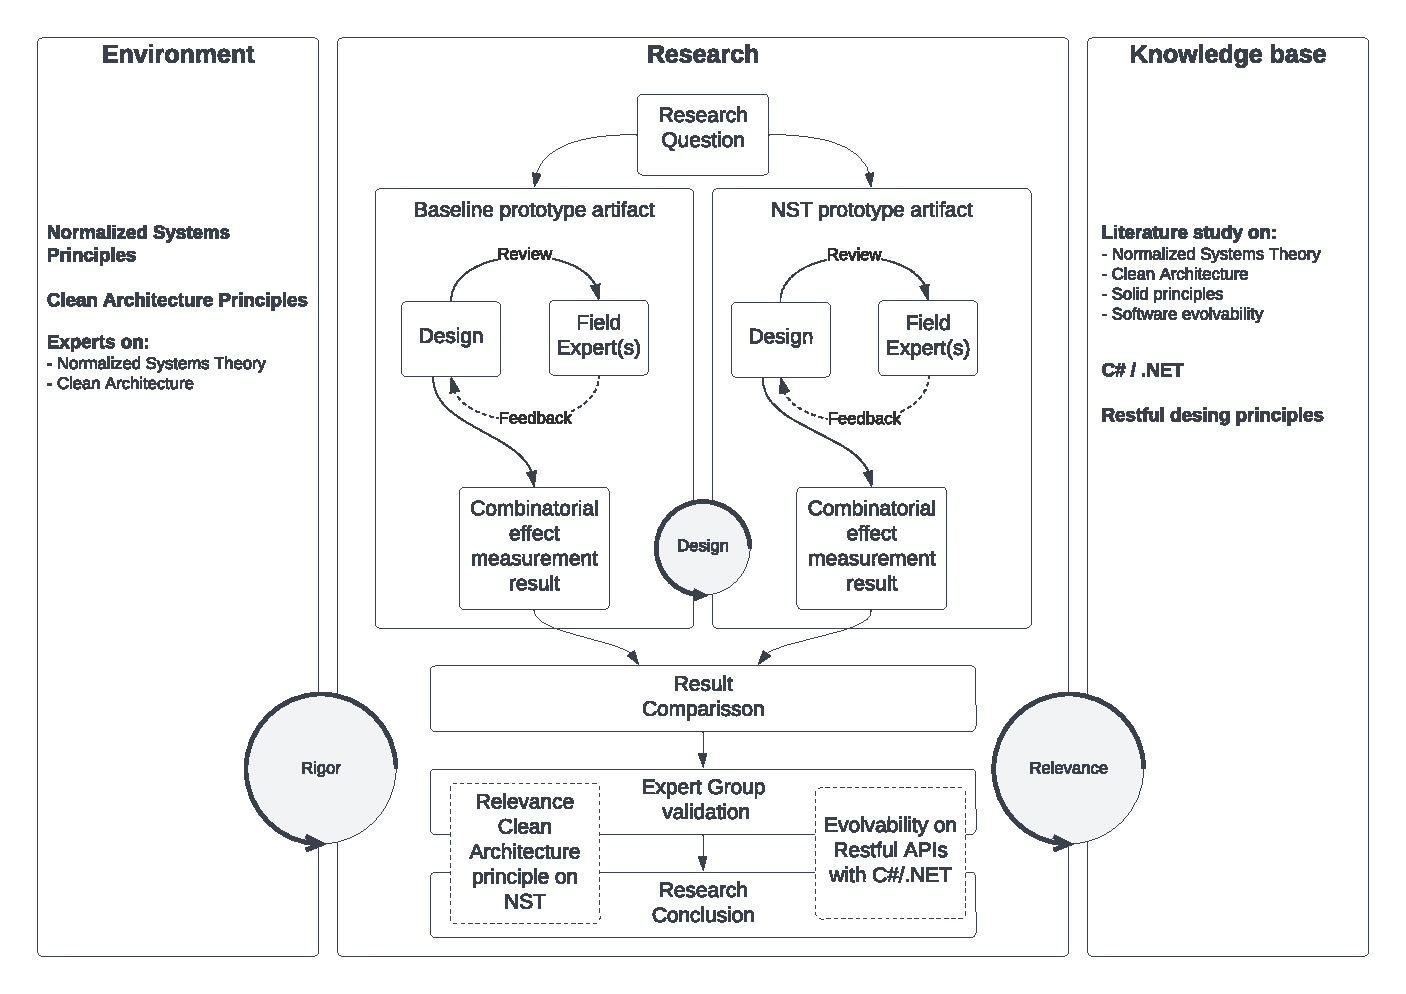
\includegraphics[width=1\textwidth]{Figures/research_approach}
    \caption[Research approach]{Research approach.}
    \label{fig:reserach_approach}
\end{figure}

The first artifact is intended to be a working prototype of a Restful API, designed
following to the Clean Architecture principles \parencite[]{martin_clean_2018} using
C\#/.NET programming language. The second artifact follows the results of the baseline
artifact. It is enhanced with the design based on the Normalized Systems Theorems. The
artifact uses the Software Generation concepts like expanding, rejuvenation and harvesting
as proposed in the paper \enquote{\citefield[]{mannaert_realization_2020}{title}}
\parencite[]{mannaert_realization_2020}

Each artifact will endure a review cycle done by field experts of on each of the given
design principles. The review cycle is used to ensure that the design and implementation
are according to those design principles.

Besides the review of the field experts, the artifacts will also be validated by using an automated
instrument (script) that measures the number of combinatorial effects on both of the
artifacts. The combinatorial effects are measured in a spectrum of changes in different
area's of the artifacts. For example:
\begin{itemize}
    \item {A change in a data entity}
    \item {A change in a use case}
    \item {A change in an action}
    \item {A change in a validation}
    \item {etc...}
\end{itemize}

The outcome of the measurements on combinatorial effects on both artifacts are the basis
for the comparison results. These results will be discussed and validated by a control
group determining the effect on the evolvability when using the Normalized Systems
Theorems in a C\#/.NET restful API. 

%\include{Chapters/Chapter4} 
%\include{Chapters/Chapter5} 

%----------------------------------------------------------------------------------------
%	THESIS CONTENT - APPENDICES
%----------------------------------------------------------------------------------------

\appendix % Cue to tell LaTeX that the following "chapters" are Appendices

% Include the appendices of the thesis as separate files from the Appendices folder
% Uncomment the lines as you write the Appendices

% Appendix A

\chapter{Appendix 1} % Main appendix title

\label{AppendixA} % For referencing this appendix elsewhere, use \ref{AppendixA}

\section{How do I change the colors of links?}

The color of links can be changed to your liking using:

{\small\verb!\hypersetup{urlcolor=red}!}, or

{\small\verb!\hypersetup{citecolor=green}!}, or

{\small\verb!\hypersetup{allcolor=blue}!}.

\noindent If you want to completely hide the links, you can use:

{\small\verb!\hypersetup{allcolors=.}!}, or even better: 

{\small\verb!\hypersetup{hidelinks}!}.

\noindent If you want to have obvious links in the PDF but not the printed text, use:

{\small\verb!\hypersetup{colorlinks=false}!}.

%% Appendix A

\chapter{Appendix 2} % Main appendix title

\label{AppendixB} % For referencing this appendix elsewhere, use \ref{AppendixA}

\section{HSome title for an appendix?}

\lipsum[2-4]

%\include{Appendices/AppendixC}

%----------------------------------------------------------------------------------------
%	BIBLIOGRAPHY
%----------------------------------------------------------------------------------------

\printbibliography[heading=bibintoc]

%----------------------------------------------------------------------------------------

\end{document}  
